% !TeX spellcheck = en_GB
%\begin{landscape}
	\begin{figure}[h!]
		\centering
		% 21/12
		\begin{subfigure}[b]{0.49\textwidth}
			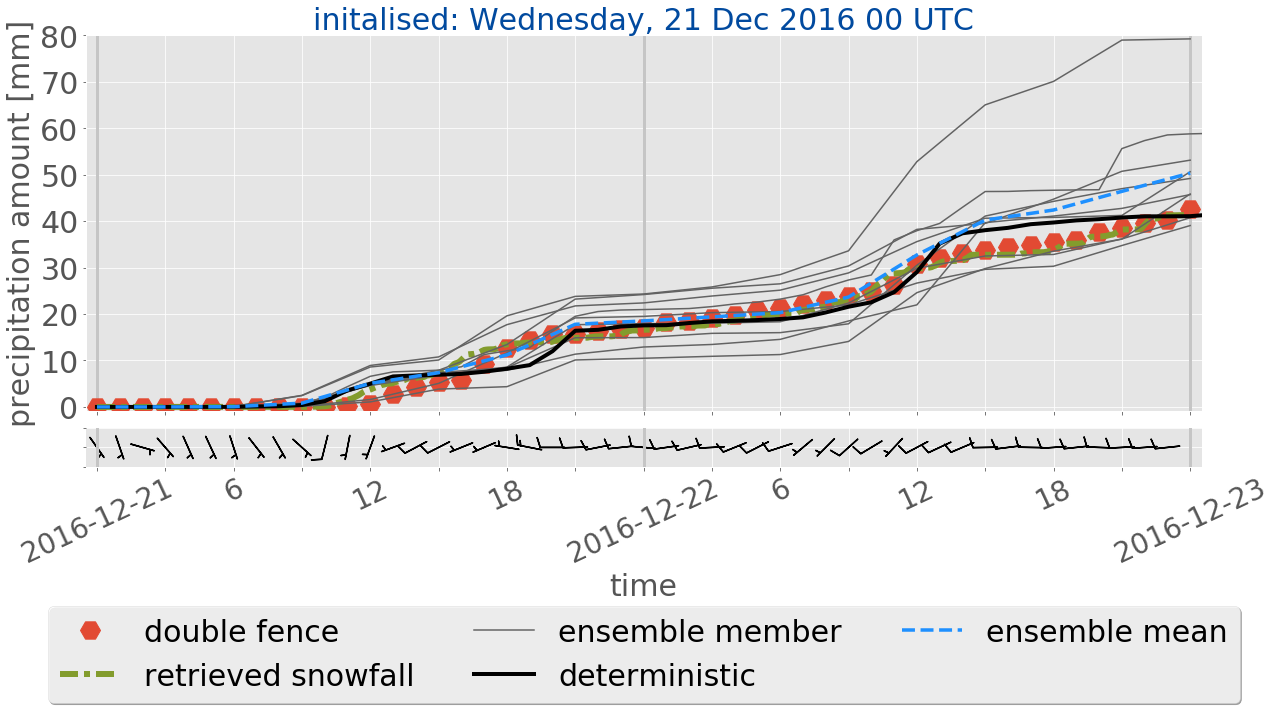
\includegraphics[width=\textwidth]{./fig_sfc_acc/acc_wind_20161221_00}
			\caption{}\label{fig:sfc_acc21}
		\end{subfigure}
        % 22/12
		\begin{subfigure}[b]{0.49\textwidth}
			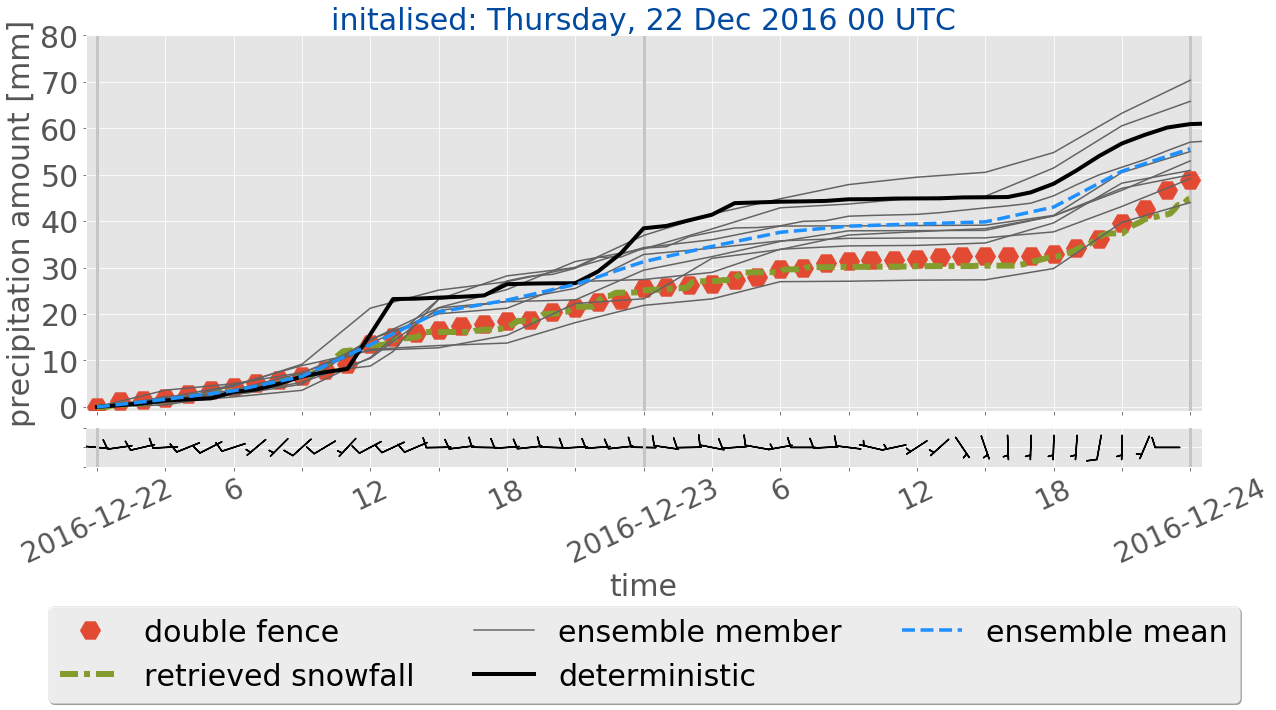
\includegraphics[width=\textwidth]{./fig_sfc_acc/acc_wind_20161222_00}
			\caption{}\label{fig:sfc_acc22}
		\end{subfigure}
	\end{figure}
    \begin{figure}\ContinuedFloat
        % 23/12
		\begin{subfigure}[b]{0.49\textwidth}
			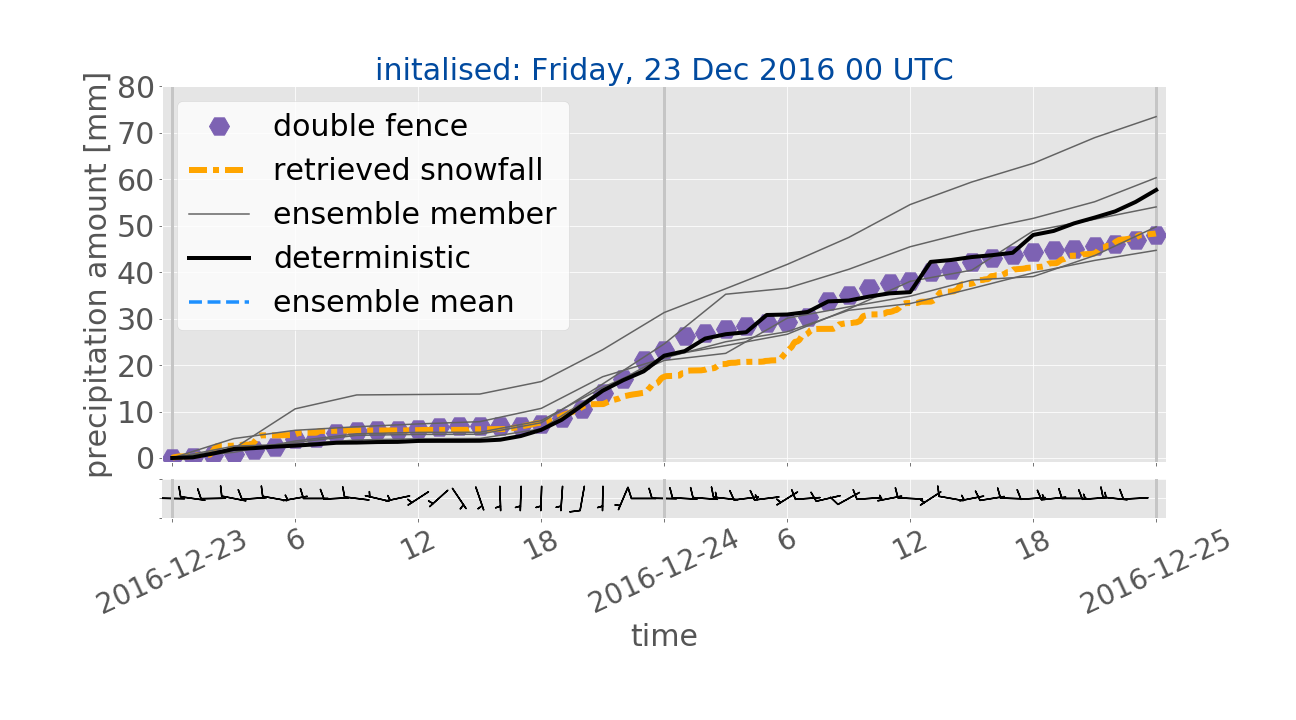
\includegraphics[width=\textwidth]{./fig_sfc_acc/acc_wind_20161223_00}
			\caption{}\label{fig:sfc_acc23}
		\end{subfigure}
        % 24/12
		\begin{subfigure}[b]{0.49\textwidth}
			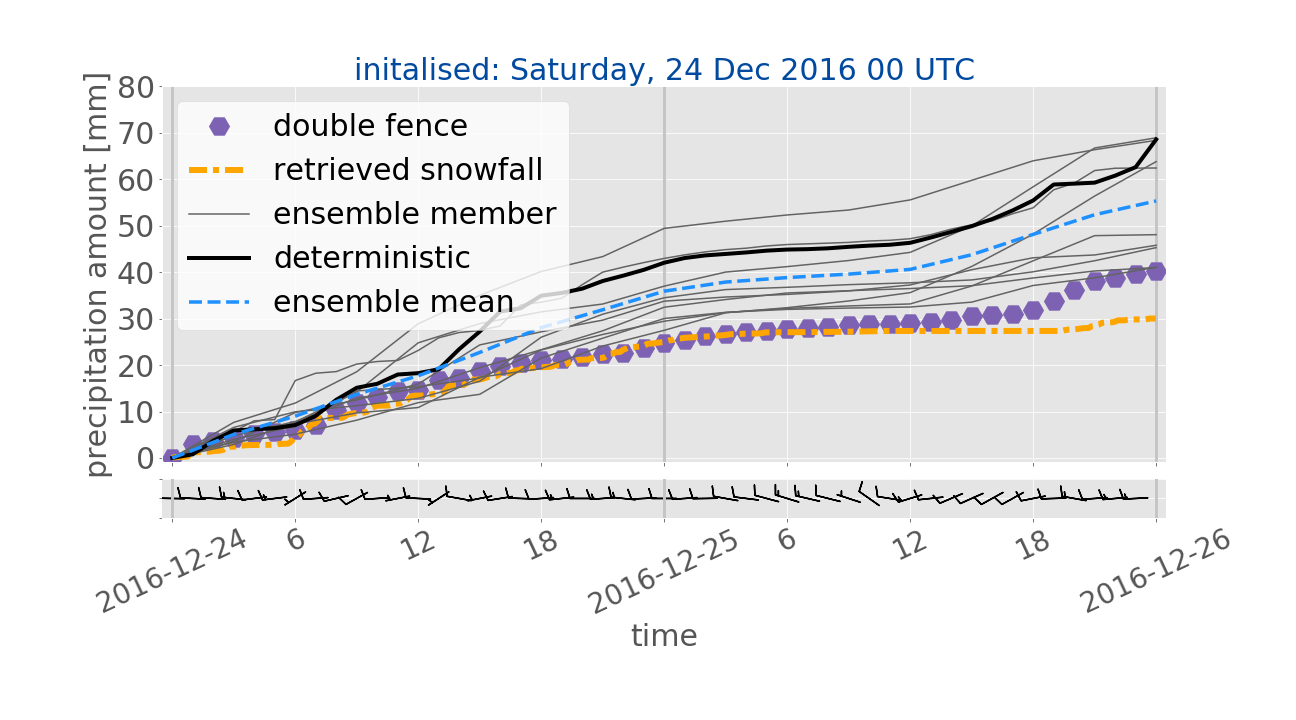
\includegraphics[width=\textwidth]{./fig_sfc_acc/acc_wind_20161224_00}
			\caption{}\label{fig:sfc_acc24}
		\end{subfigure}
        % 25/12
		\begin{subfigure}[b]{0.49\textwidth}
			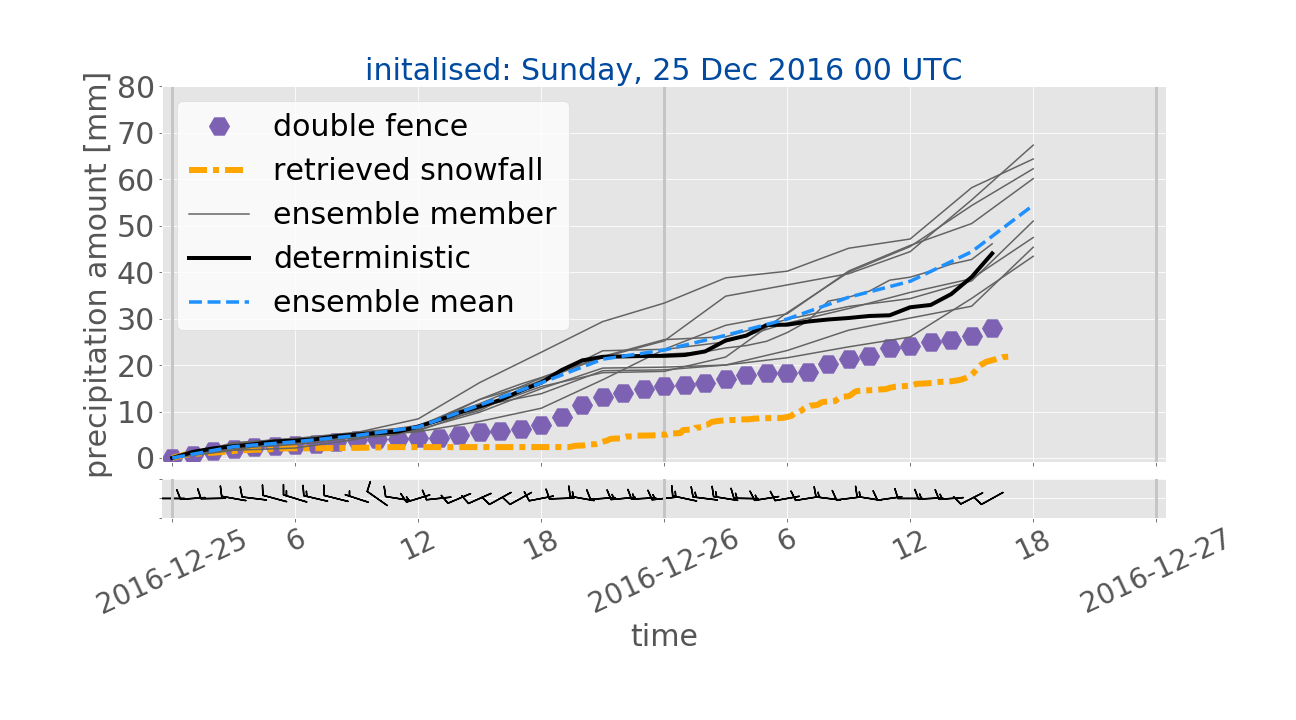
\includegraphics[width=\textwidth]{./fig_sfc_acc/acc_wind_20161225_00}
			\caption{}\label{fig:sfc_acc25}
		\end{subfigure}
        % 26/12
		\begin{subfigure}[b]{0.49\textwidth}
			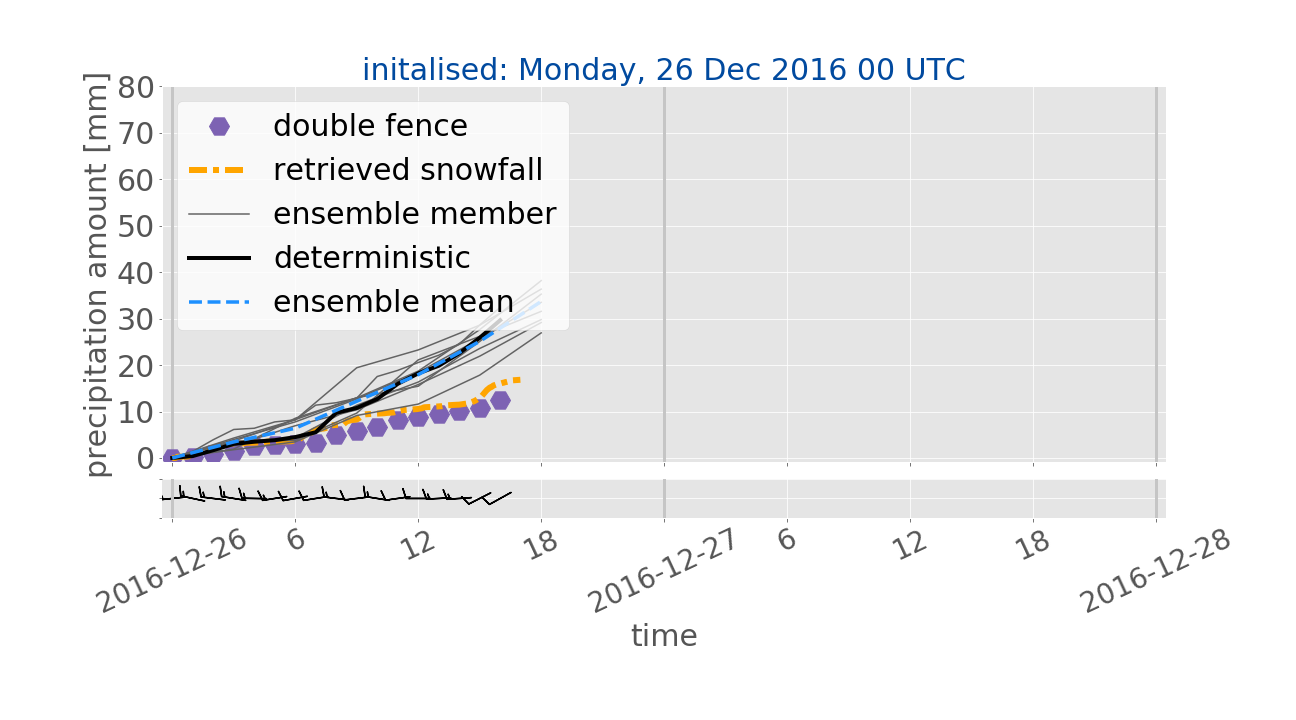
\includegraphics[width=\textwidth]{./fig_sfc_acc/acc_wind_20161226_00}
			\caption{}\label{fig:sfc_acc26}
		\end{subfigure}
    \caption{Surface snowfall accumulation. Representing the values from the double fence in light blue, hexagons; optimal estimation retrieval output at snow layer height \SI{800}{\metre} in dashed orange; and ensemble member deterministic forecast, initialised at \SI{00}{\UTC} in black and its nine perturbed ensemble members in grey. Underneath are the associated wind barbs from the deterministic MEPS forecast and the weather mast at \SI{10}{\metre} height. }\label{fig:sfc_acc}
	\end{figure}

	
